The matching consist on link objects between both images. It's an essential step in the algorithm because without step is not possible to track rightly 3D targets.\\

\begin{figure} [h]
	\centering
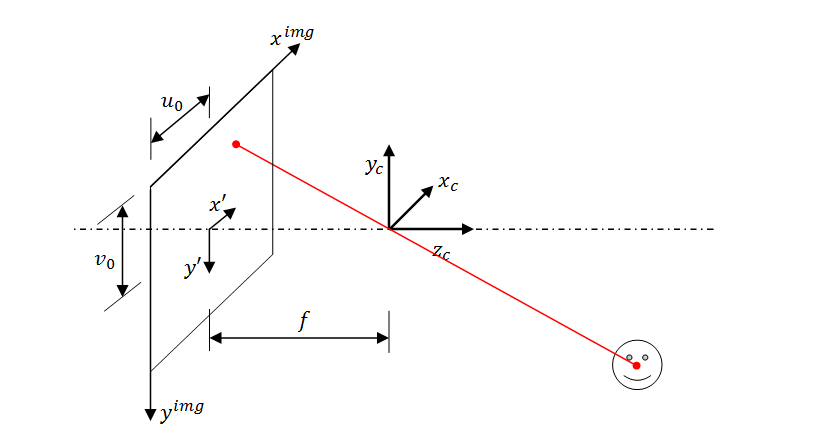
\includegraphics[width=0.75\textwidth,natwidth=544,natheight=388]{../Images/c1/pinhole_model.png} 
	\caption{Pinhole Camera Model}
	\label{fig:Pinhole_Model}
\end{figure}

Firstly, in this article it's assumed that camera's behavior is governed by the pinhole model. According to this and assuming that the X axis of the camera define its the orientation, every space point (X,Y,Z) has the following projection. \\

\begin{align}
X^{img} = f*\frac{Y}{X} \\
Y^{img} = f*\frac{Z}{X}
\end{align}

Where f is the focal lenght of the camera; $X^{img}$ and $Y^{img}$ are the projection of the three dimensional point on the camera plane. This equations are in $\mathbb{R}^3$ the ecuations of 2 planes that cut in one line (The epipolar line). So in conclusion, every segmented object in the camera's images provide a pair of planes (or a single line). Ideally, if the Segmentation had no errors every pair os lines (One per camera for the same target) will cross in a point. However due to errors is almost improbable. That's why the matching algorithm links the objects by minimizing the distance between lines.

\begin{figure}[h]
\centering
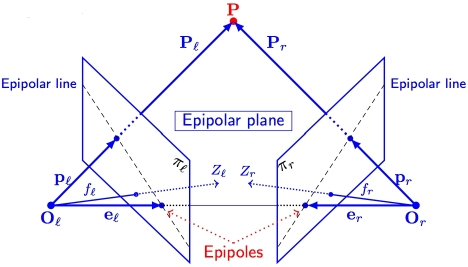
\includegraphics[width=0.75\textwidth,natwidth=468,natheight=267]{../Images/c1/Epipolar_Lines.png}
\caption{Epipolar Lines}
\label{fig:Epipolar_Lines}
\end{figure}

To be precise, the obtained image in the computer hasn't got negative projection. The values on the image are displaced vertically and horizontally. This displacement is stored as the camera�s image centroid or $(u_0, v_0)$. Eventually, equations are: \\

\begin{align}
X^{img} = f*\frac{Y}{X} + u_0 \\
Y^{img} = f*\frac{Z}{X} + v_0
\end{align}
